% $ platex body
% $ dvipdfmx body

\documentclass[a4j]{jarticle}

\title{「データ解析入門」レポート}
\author{1677281 山内 拓弥}
\usepackage{colortbl}
\usepackage[dvipdfmx]{graphicx}
\renewcommand{\thesection}{課題\arabic{section}}
\renewcommand{\thesubsection}{}

\begin{document}

\maketitle

\section{}
クラスタリングとベクトル量子化の定義を、
その違いがわかるように説明し、
平方和最小基準クラスタリング問題と2乗誤差に基づくベクトル量しか問題の
局所最適解における性質について記述しなさい。

\subsection{【回答】}
TBD

\section{}
教科書の「HokkaidoTowns\_xy\@.dat」データを、 k-meansアルゴリズムと競合学習で、
6分割にクラスタリングする実験を行い、 その結果を示し、考察しなさい。
具体的には、プログラムに与える引数である「乱数の種」、
「学習率」(競合学習のみ)などをいくつか変更して実験を行い、
両手法の性能比較を行いなさい。

\subsection{【回答】}

\paragraph{乱数の種を振り、k-meansアルゴリズムと競合学習を比較}

\begin{table}[h]
 \begin{center}
  \begin{tabular}{|r||r|r|r|} \hline
            & k-means     & \multicolumn{2}{|c|}{競合学習} \\ \cline{2-4}
   試行番号 & $E_Q = J_W$                  & $E_Q$  & $J_W$  \\ \hline \hline
          1 &                       474825 & 472490 & 472288 \\ \hline
          2 & \cellcolor[gray]{0.8} 543956 & 472673 & 472217 \\ \hline
          3 &                       474825 & 472577 & 472288 \\ \hline
          4 & \cellcolor[gray]{0.8} 609216 & 472959 & 472808 \\ \hline
          5 &                       473367 & 472557 & 472288 \\ \hline
          6 &                       473367 & 472501 & 472288 \\ \hline
          7 &                       472288 & 472439 & 472217 \\ \hline
          8 & \cellcolor[gray]{0.8} 503663 & 472648 & 472288 \\ \hline
          9 &                       472769 & 472429 & 472288 \\ \hline
         10 &                       474818 & 472367 & 472217 \\ \hline
  \end{tabular}
 \end{center}
\end{table}

\begin{figure}[tbp]
 \begin{minipage}{0.5\hsize}
  \begin{center}
   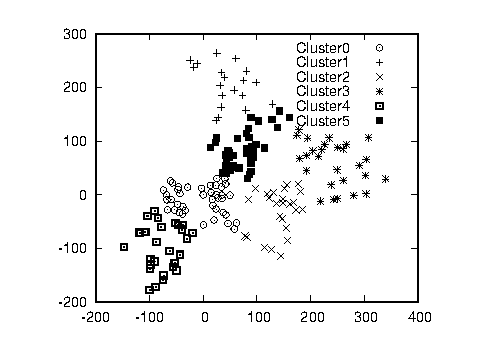
\includegraphics[width=\hsize]{fig/Hokkaido_xyl_seed1.eps}
  \end{center}
  \caption{k-meanアルゴリズム、良い結果}
  \label{fig:k-mean-seed1}
 \end{minipage}
 \begin{minipage}{0.5\hsize}
  \begin{center}
   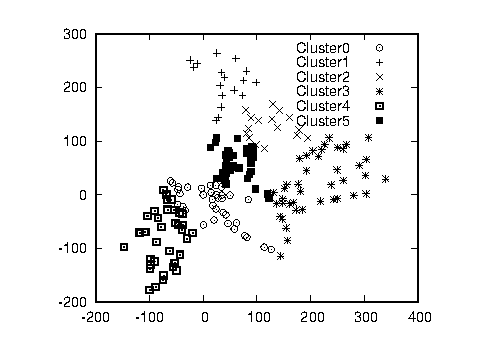
\includegraphics[width=\hsize]{fig/Hokkaido_xyl_seed4.eps}
  \end{center}
  \caption{k-meanアルゴリズム、悪い結果}
  \label{fig:k-mean-seed4}
 \end{minipage}
\end{figure}

\paragraph{競合学習の結果}

\begin{figure}[tbp]
 \begin{minipage}{0.5\hsize}
  \begin{center}
   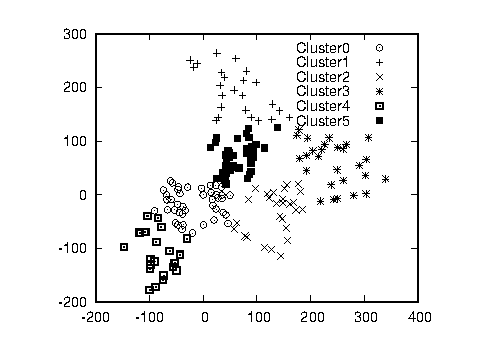
\includegraphics[width=\hsize]{fig/Hokkaido_xyl_compLearn.eps}
  \end{center}
  \caption{競合学習、学習率$=1$のクラスタリング結果}
  \label{fig:compLearn-map}
 \end{minipage}
 \begin{minipage}{0.5\hsize}
  \begin{center}
   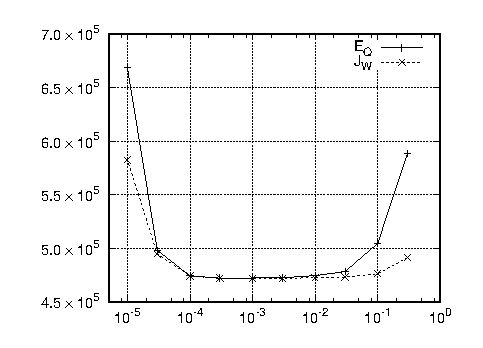
\includegraphics[width=\hsize]{fig/compLearn.eps}
  \end{center}
  \caption{競合学習、学習率と$E_Q$、$J_W$}
  \label{fig:compLearn}
 \end{minipage}
\end{figure}

\section{}
教科書の「HokkaidoTowns\_xy\@.dat」データを、
k-meansアルゴリズムなどで6分割したクラスタリングを行い、
その結果を「Hokkaido\_xyl\@.dat」としなさい。
次に、修正パーセプトロン学習プログラムであるmodPerceptronを用い、
上記クラスタリング結果を学習パターンとして学習させなさい。
その時、「乱数の種」、「学習率」を変化させて実験し、
収束するまでの繰り返し回数の傾向について考察しなさい。

\subsection{【回答】}
TBD

\section{}
教科書の「HokkaidoTowns\_xy\@.dat」の各カラムがx y座標の座標値を表すとします。
このデータの重みベクトルによるボロノイ分割が、
y軸を境界とする2分割になりました。
この重みベクトルはどのようなものになるか例を使って説明しなさい。

\subsection{【回答】}
TBD

\section{}
赤と青の2つの箱があり、
赤の箱にはりんごが2個とオレンジが6個、
青の箱にはりんごが3個とオレンジが1個入っているとする。
箱の1つをランダムに選び、果物をランダムに1個取り出す。
その際、赤の箱を40\%、青の箱を60\%選び、
箱の中の果物は別け隔てなく同じ確からしさで選ぶ。
この時、オレンジを選び出したとして、
それが青い箱から取り出されたものである確率はいくらか?
導出過程も含めて書きなさい。

\subsection{【回答】}
TBD

\section{}
教科書の表5\.2「フルーツのブレンド割合」の値は、
壷を選んだときに各フルーツが取り出される条件付確率を表しています。
今、各壷が選ばれる確率がすべて等しいとします。
この時、下記のフルーツポンチがあるとき、
それぞれの壷が選ばれたという「対数事後確率の大小関係を比較できる値」
を求め比較しなさい。

\subsection{【回答】}
TBD

\section{}
フルーツポンチをgenPunchで生成し、
それをestParamで処理して、
モデルのパラメータを推定する実験をしなさい。
ボウルの数や果物の数を変えると、
推定結果の精度にどのような影響があるかについて考察しなさい。

\subsection{【回答】}
TBD

\end{document}
